\section{Design Rationale and System Overview}
\label{sec:overview}

\begin{figure}[!t]
       \vspace{2mm}
        \begin{minipage}{1\linewidth}
        \centering    
        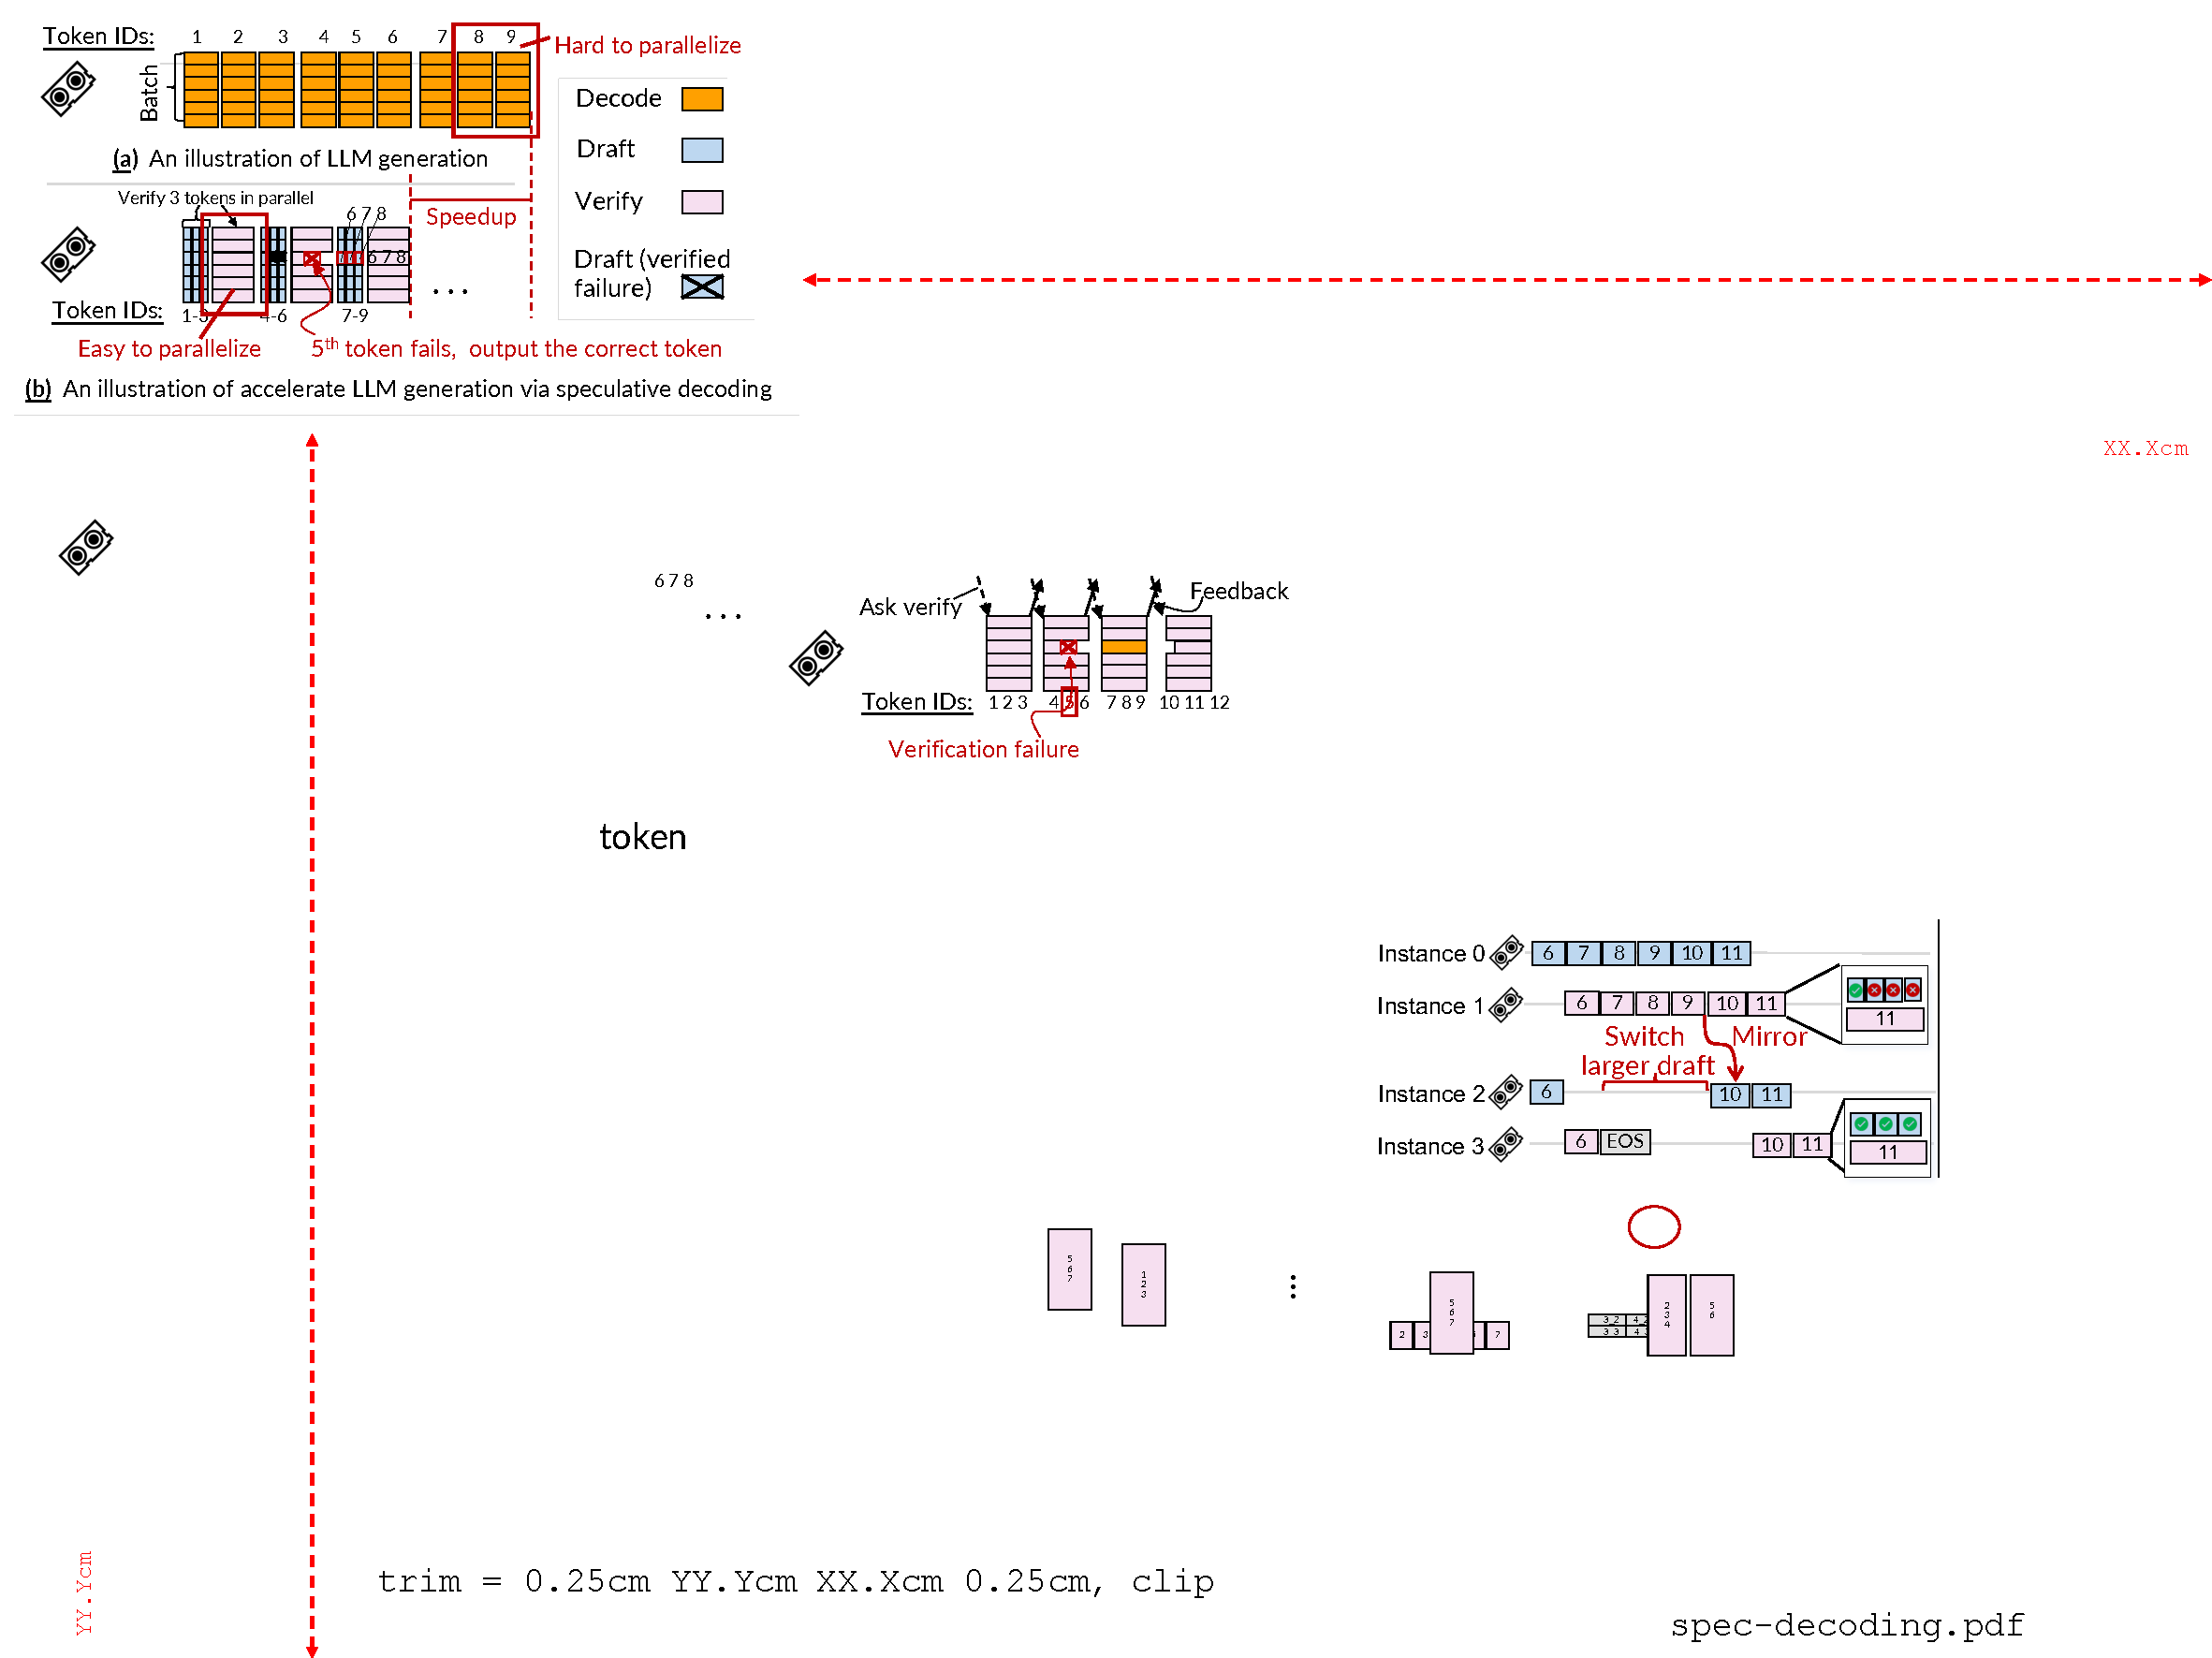
\includegraphics[width=0.95\linewidth, trim=0.25cm 22.4cm 26.6cm 0.25cm, clip]{figs/spec-decoding.pdf} 
        \end{minipage} \\[2pt]
        \begin{minipage}{1\linewidth}
        \caption{\small{%
        An illustration of speculative decoding.  
        }}
        \label{fig:spec-decoding}
        \end{minipage} \\[-15pt]
        \end{figure} 

\nospacestitle{Opportunity: speculative decoding for rollout}~\cite{DBLP:journals/corr/abs-2302-01318,DBLP:conf/icml/LeviathanKM23,eagle-3,turbospec,DBLP:conf/nips/SternSU18,DBLP:conf/asplos/MiaoOZCWZWZYSSC24}.
It is a common technique to accelerate sequential LLM generation:
As detailed in \fig{fig:spec-decoding} (a),
the original generation iteratively generates tokens for the current batch
using the model being trained. 
With speculative decoding (b),
we first generate a sequence of tokens using a fast draft method,
e.g., with a smaller model, as detailed in \textsection{\ref{sec:design-decouple}}.
The drafted tokens are then verified by the trained model 
before being accepted as the generated tokens.

Since the verification can be performed on multiple tokens in parallel,
its time is similar to or less than that of generating a single token if GPU computation is not the bottleneck. 
Thus, if tokens are accepted, speculative decoding is much faster than the original generation,
as shown in the right half of \fig{fig:rollout-schedule} (b).
On the other hand, if the verification rejects the drafted tokens,
e.g., the 5$^{th}$ token for request 3 in our example,
the rejected token and draft tokens after it,
e.g., tokens 5--6, will be discarded, and the drafter starts
from token 6---as the verification will provide a correct 5$^{th}$ token.


\stitle{Challenge \#1: Limited speedup for typical training configurations. \,}
While intuitive, we found adopting state-of-the-art speculative decoding techniques\cite{pld,lookahead,eagle-2,specinfer}
in rollout results in limited speedup,
because the speculation verification is inefficient on 
per-worker batch sizes common in training (see {\fig{fig:rollout-schedule}} (a)). 
{\fig{fig:motiv-batchsize}} (a) shows the distribution of per-worker batch sizes collected
from production post-training jobs, and 
(b) compares the time of generation at most {4,096} tokens 
using speculative decoding and the original generation
on a {Qwen2.5-32B} model.
We can see that for common per-worker batch sizes (e.g., 128), speculative decoding brings no
or negative gain.
The reason is that the verification time increases more significantly 
with the increased request batch size than others,
as shown in {\fig{fig:rollout-schedule}} (d), 
because verification introduces a larger token batch 
than original generation.


\begin{figure}[!t]
        \vspace{2mm}
        \begin{minipage}{1\linewidth}
        % \hspace{2mm}
        \centering    
        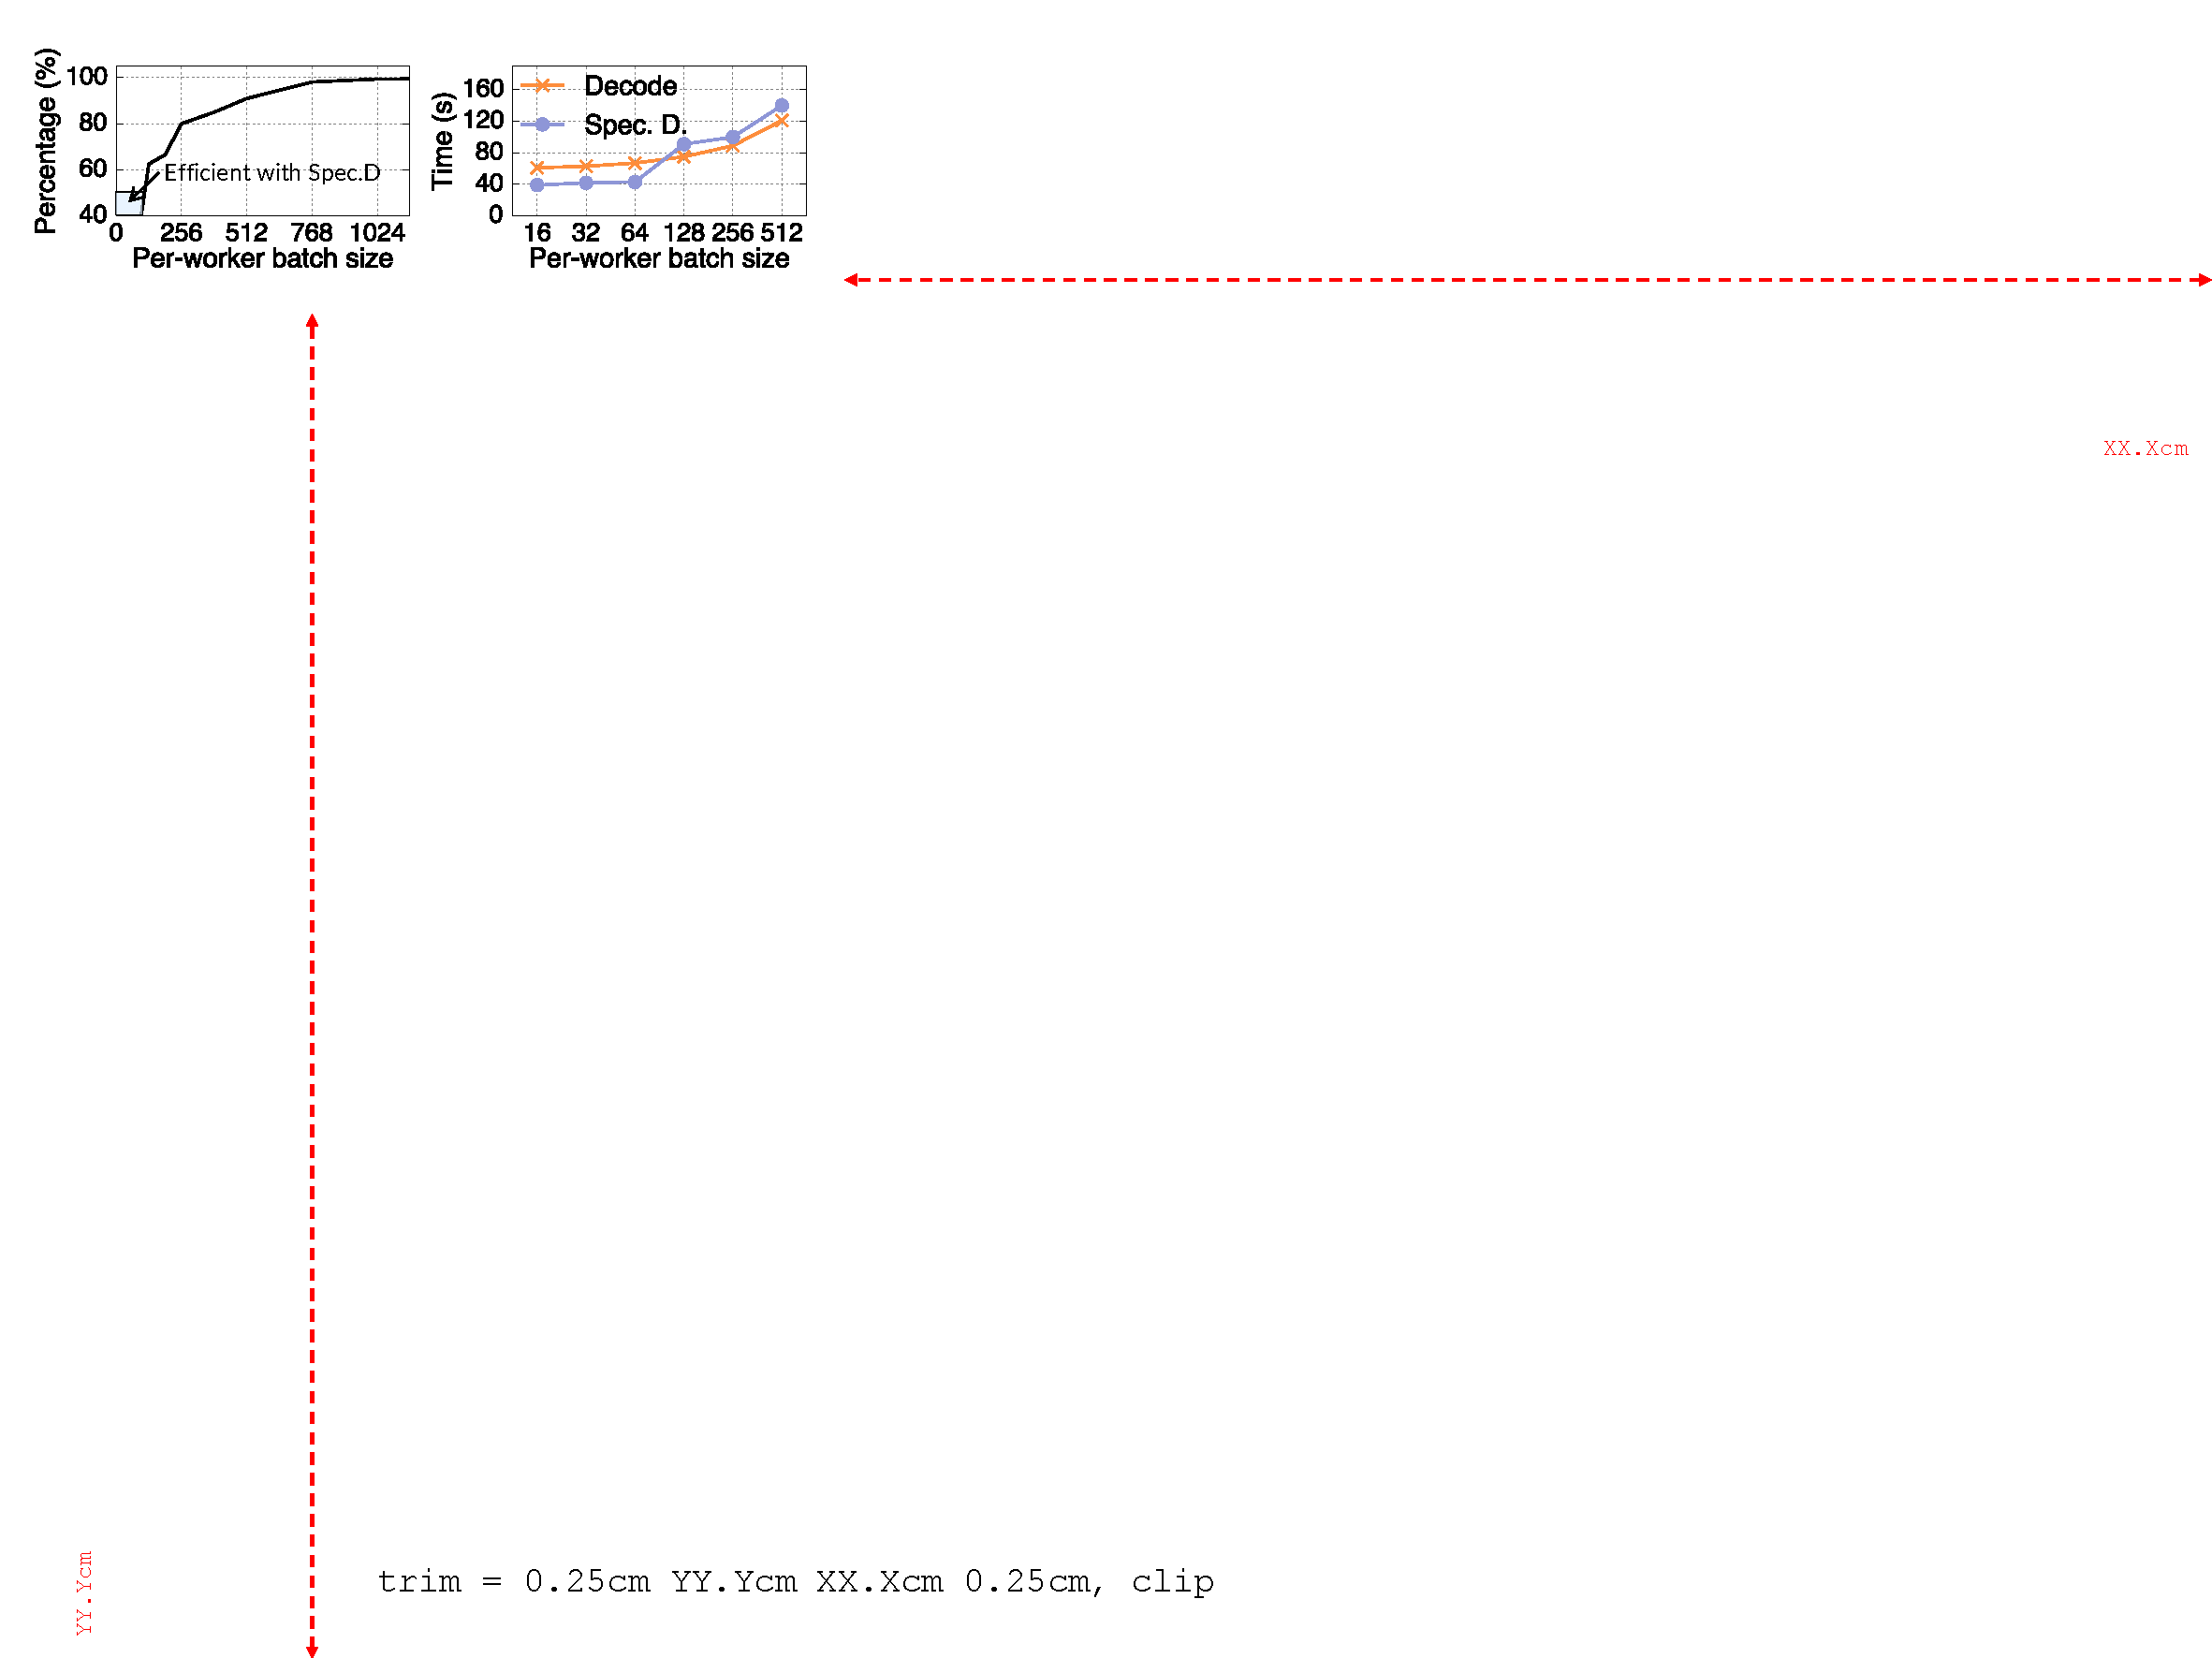
\includegraphics[width=1\columnwidth,trim=0.25cm 24.37cm 24.8cm 0.25cm, clip]{figs/motiv-batchsize.pdf} \\[3pt]
        \end{minipage} \\[0pt]
        \begin{minipage}{1\linewidth}
        \caption{\small{%
        {
            (a) Distribution of the initial per-worker batch sizes of post-training traces in the last 6 
            months in a large production cluster. 
            (b) The acceleration of speculative rollout given such a batch size
            on a {Qwen2.5-32B} checkpoint. 
        }}}
        \label{fig:motiv-batchsize}
        \end{minipage} \\[-5pt]
\end{figure}

One may notice that the per-worker batch size decreases during rollout 
as more requests finish.
% However, we found that at least {20\,\%} of the rollout time
% is executed under relatively large batch sizes
However, in at least 20\% of the rollout time, 
the batch size is relatively large
in our DAPO-32B-20K trace (see \textsection{\ref{sec:eval-setup}}),
which still calls for efficient speculative decoding acceleration.
In training, even a tiny acceleration matters due to the
potential of saving many GPU hours.

\begin{figure}[!t]
        \vspace{4mm}
        \begin{minipage}{1\linewidth}
        % \hspace{2mm}
        \centering    
        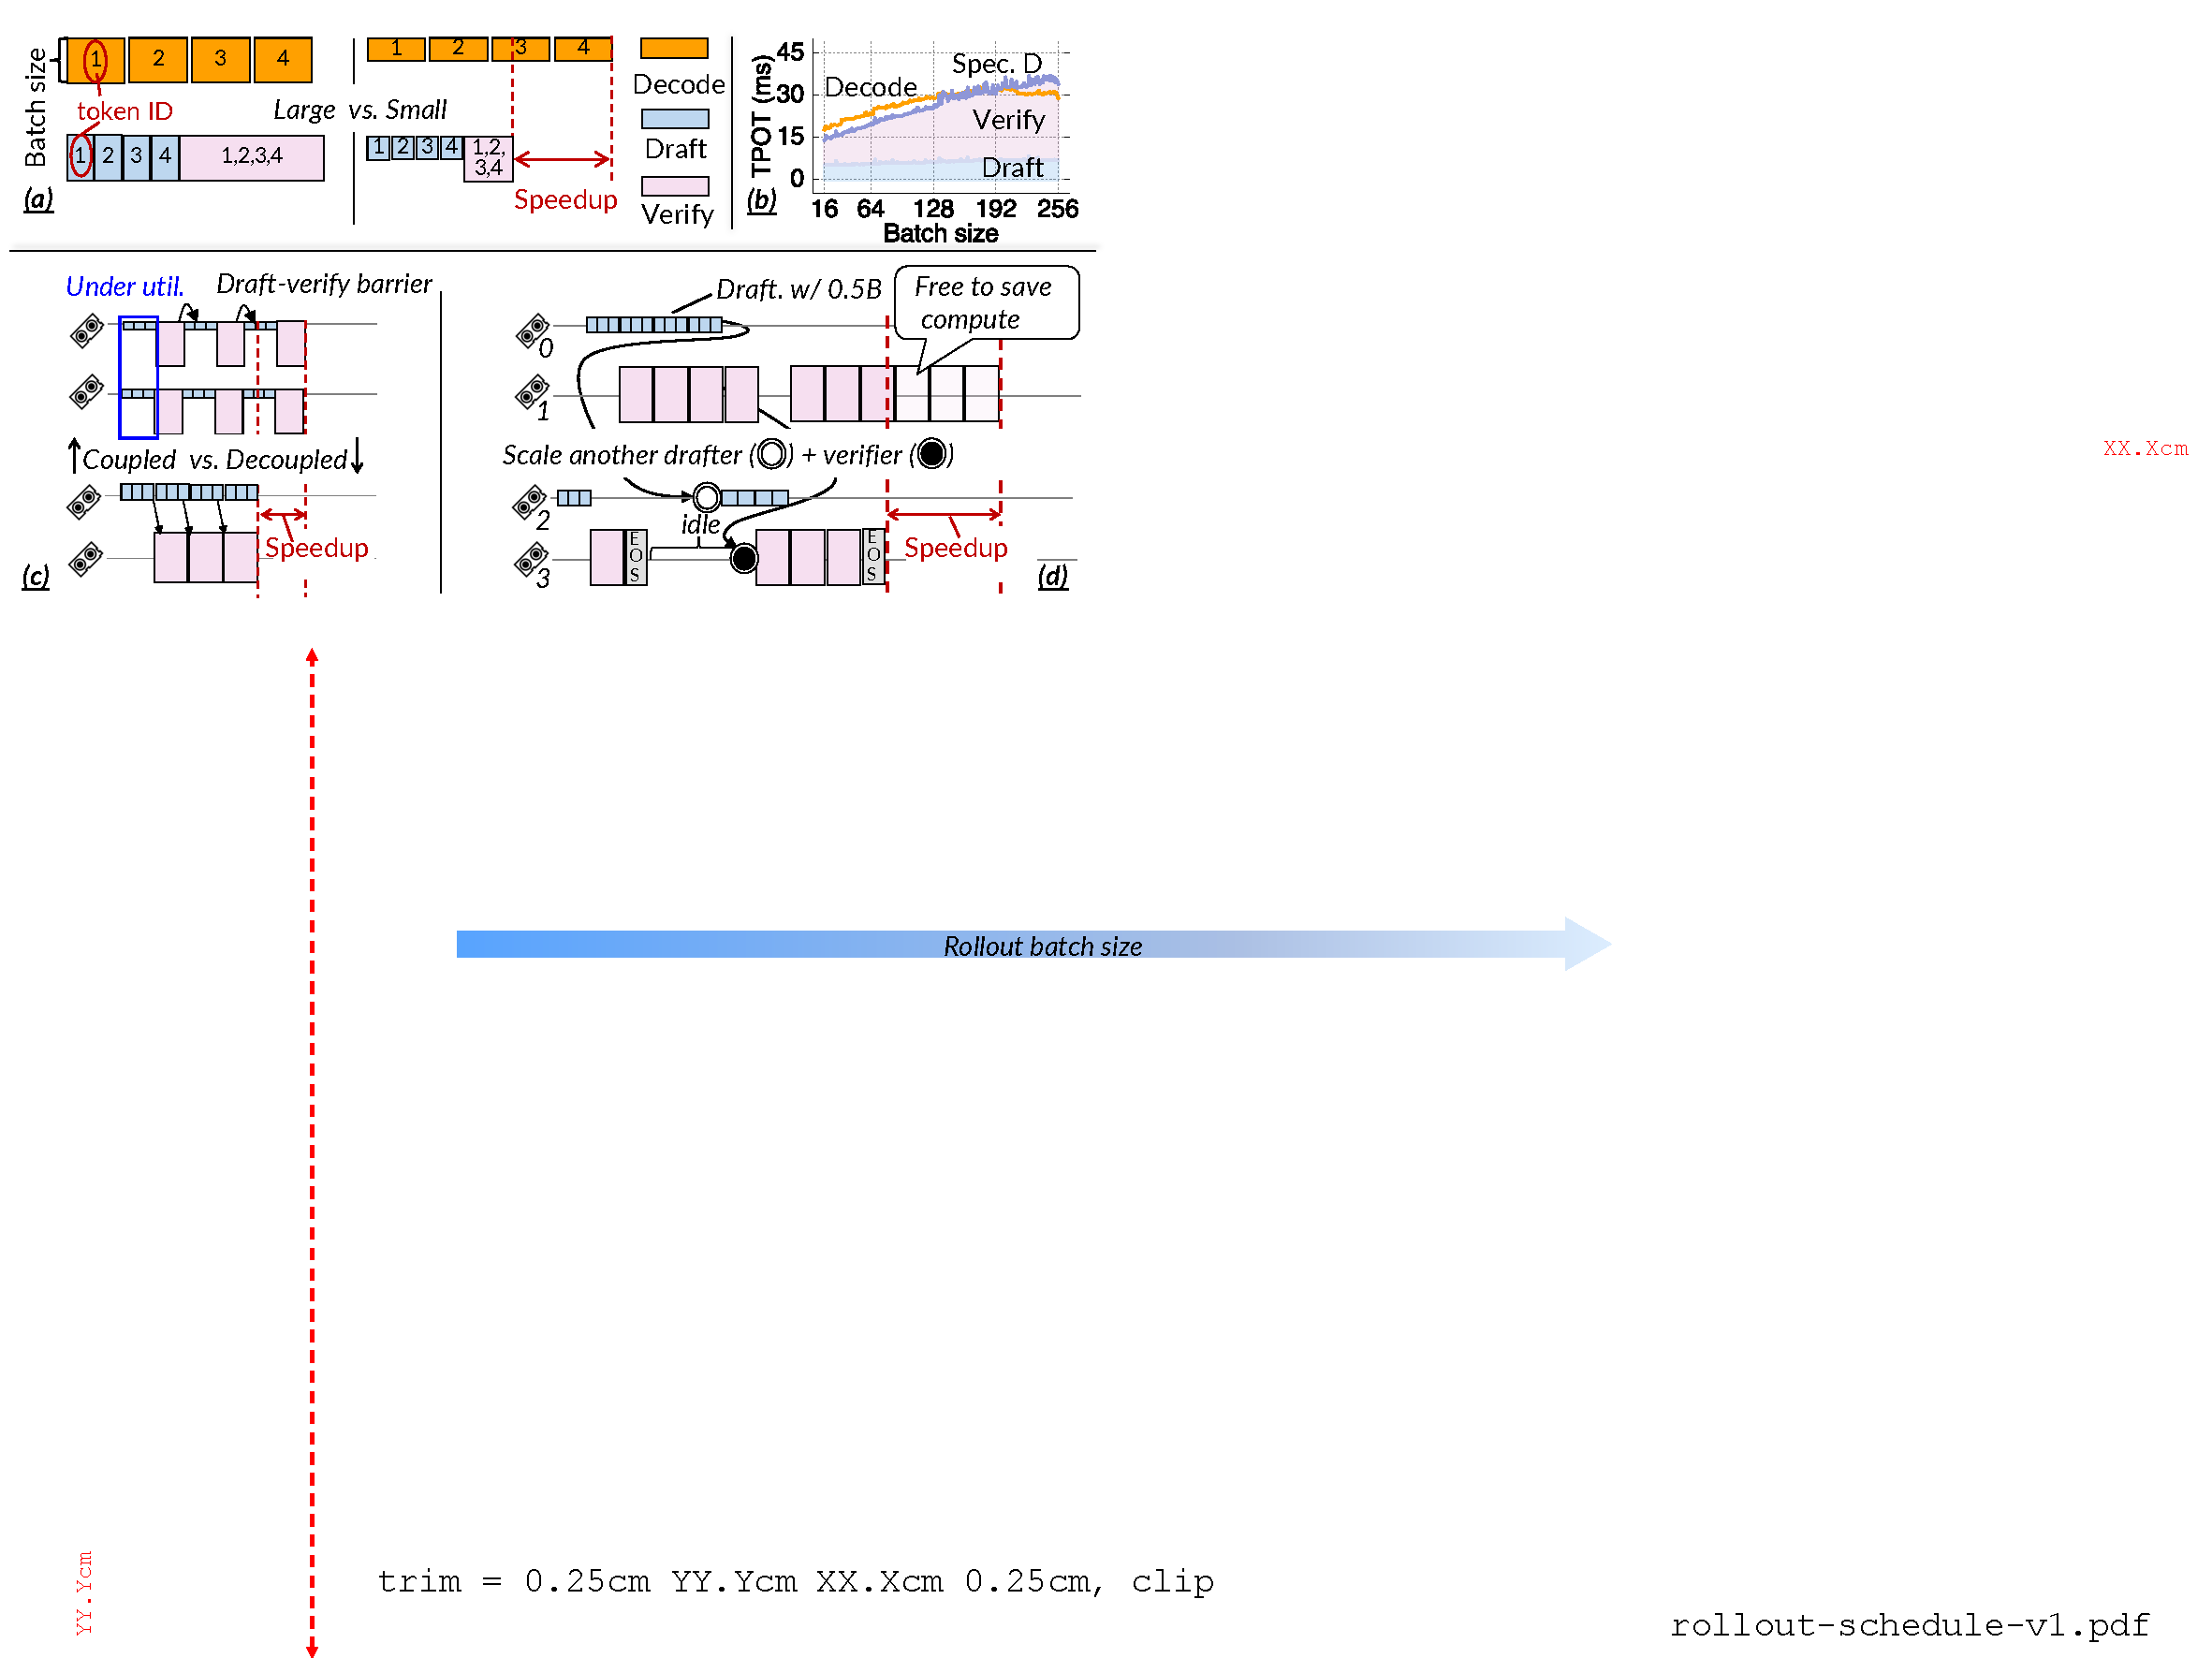
\includegraphics[width=0.9\linewidth, trim=0.25cm 18.4cm 20.35cm 0.25cm, clip]{figs/rollout-schedule-v2.pdf}
        % \hspace{2mm}
        \end{minipage} \\[1pt]
        \begin{minipage}{1\linewidth}
        \caption{\small{%
        (a) An illustration of the limited speedup of speculative decoding with
        increased verification costs due to increased batch size.
        (b) A TPOT (Time Per Output Token) analysis of speculative and
        normal decoding of Qwen2.5-32B with different batch sizes.
        (c) An illustration of how decoupled execution reduces GPU underutilization
        due to the drafter.
        (d) An illustration of how Fastest-of-N speculation works with finished batches.
        }}
        \label{fig:rollout-schedule}
        \end{minipage}
        \end{figure} 

\etitle{Our solution: decoupled speculation (\textsection{\ref{sec:design-decouple}}). \,}
As we have mentioned in the introduction, we decouple the dependency between
drafting and verification,
which allows us to fully utilize GPUs for speculative decoding.
As shown in {\fig{fig:rollout-schedule}} (c),
unlike traditional coupled execution where the drafter must wait for the verifier,
we (1) distribute the drafter and verifier to separate GPUs and
(2) allow the drafter to aggressively continue without waiting for the verifier.
Such an execution scheme provides more GPU time to the verifier
because we only need to allocate a few GPUs for the drafter
to avoid many GPU executions being GPU-underutilized during drafting.
Note that for the same set of GPUs, decoupled execution increases
the per-worker batch size for the verifier:
in our example, the batch size is doubled.
This does not offset the gain brought by decoupling because
verification with a 2\,$\times$ batch (from 128 to 256)
only incurs a 1.4\,$\times$ higher latency (as shown in {\fig{fig:rollout-schedule}} (b)).
Besides, our placement method further minimizes the cost by configuring
an appropriate parallelism that 
distributes the verification across more GPUs.


Decoupled speculative decoding faces the challenge of wasting more GPU resources upon 
possible decreased acceptance rates. 
In the example in {\fig{fig:rollout-schedule}} (c),
if a token in positions 1--3 is mis-speculated, extra drafted tokens (4--6) will be discarded,
which could not happen in a coupled speculation. 
Fortunately, we found it has little impact on many requests since their
acceptance rates remain high, so the speedup of decoupled execution offsets the loss due to waste,
still enabling a rapid reduction in the per-worker batch size.
To further cope with requests that suffer from significantly decreased acceptance rates,
we only relax but not fully discard the draft-verify dependency, 
using a draft window to control the aggressive generation,
i.e., the drafter is only allowed to be ahead of the verifier by a certain number of tokens.
Our per-request reconfiguration effectively adjusts these windows online
as long as we detect a significant decrease in the acceptance rate for a request.

\begin{figure}[!t]
    %    \vspace{2mm}
        \begin{minipage}{1\linewidth}
        \hspace{-1mm}
        \centering    
        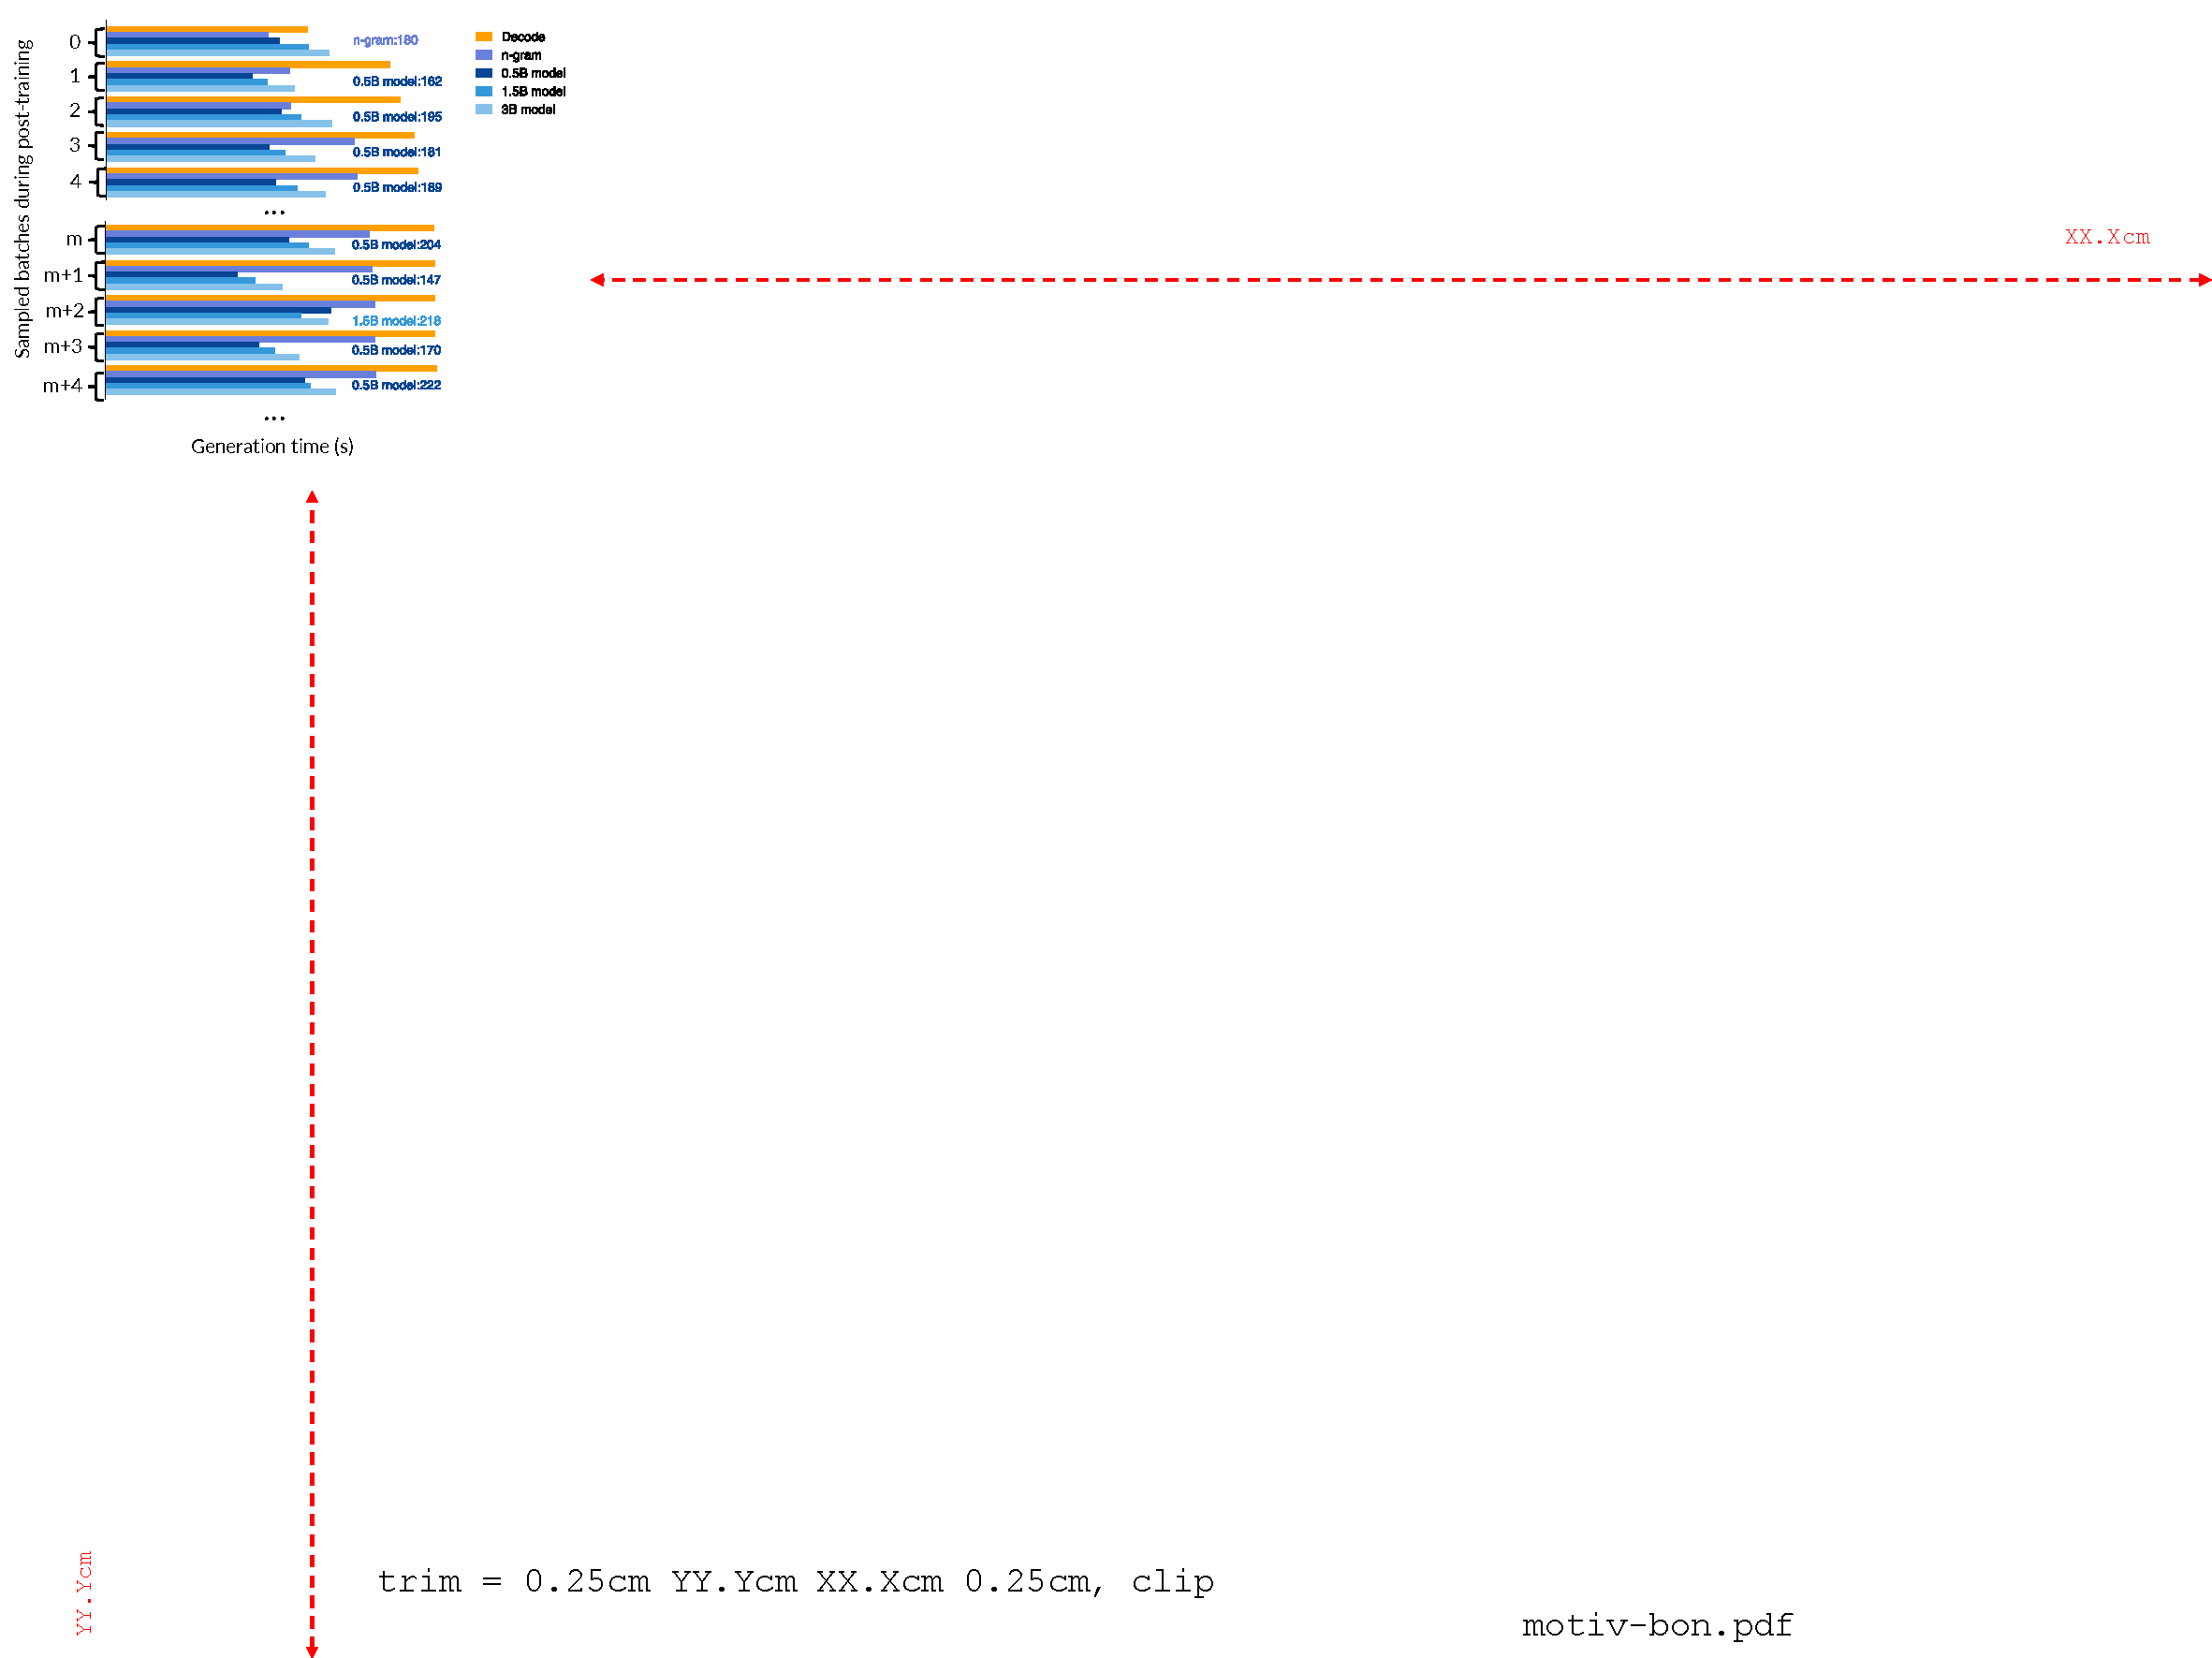
\includegraphics[width=0.85\columnwidth,trim=0.25cm 21.2cm 29.8cm 0.25cm, clip]{figs/motiv-bon.pdf} \\[3pt]
        \end{minipage} \\[-5pt]
        \begin{minipage}{1\linewidth}
        \caption{\small{%
        {
                A characterzation of the speedup of different draft methods 
                on DAPO-32B-20K (see \textsection{\ref{sec:eval-setup}}) training trace. 
        }}}
        \label{fig:motiv-bon}
        \end{minipage} \\[-15pt]
\end{figure}

\stitle{Challenge \#2: Selecting the best draft methods without priori knowledge (\textsection{\ref{sec:design-bon}}).  \,}
Selecting the best draft method is critical to ensuring high speedup yet is quite challenging
because the optimal draft method for each prompt varies and is unknown a priori.
The diversity stems from the variation in acceptance rates for a given request.
{\fig{fig:motiv-bon}} illustrates the speedup of different draft methods
on different requests from a batch collected from the training trace.
We can see that although many requests achieve the highest speedup with 0.5B drafting models,
some require 1.5B models and others require statistical methods like n-gram.
Directly executing multiple draft methods in parallel is infeasible
because it requires significantly more GPUs---not only to host multiple draft models but also to verify their outputs.
% requiring not only deploying multiple drafting models,
% but also more costly verification process to verify the outputs from multiple draft methods.

\etitle{Our solution: Fastest-of-N speculation. (\textsection{\ref{sec:design-bon}})\,}
At the start of the rollout, 
we use the profiled acceptance rate to select the estimated best draft method,
based on the observation that although each prompt's acceptance rate varies significantly,
for a large batch, 
the average acceptance rate is statistically stable.
Thus, the selection based on the average is likely to be close to the optimal for the batch.
The best draft is selected based on a ladder we constructed offline, 
which holistically considers major methods, 
including model-based~\cite{spd} and n-gram-based~\cite{pld,lookahead}. 


During the rollout, when more GPUs are freed due to finished requests,
{\sys} dynamically utilizes freed GPUs to deploy more draft methods for tailed requests,
where parallel drafting naturally approximates the best draft method better,
because as long as the fastest draft method generates all the tokens, 
we can treat the requests as finished. 
As shown in {\fig{fig:rollout-schedule}} (d),
if worker 3 becomes idle, we add the second-best draft method (1.5B)
to accelerate the unfinished requests.
Note that in the illustration we only add one more verification instance
since the drafter can be piggybacked on other workers as it is relatively lightweight.
If the 1.5B drafting model finishes earlier,
the request is completed, and the request is also removed from other workers (e.g., worker 0 and 1).

\begin{figure}[!t]
        \hspace{-1mm}
        \begin{minipage}{1\linewidth}
        \hspace{1mm}
%        \centering    
        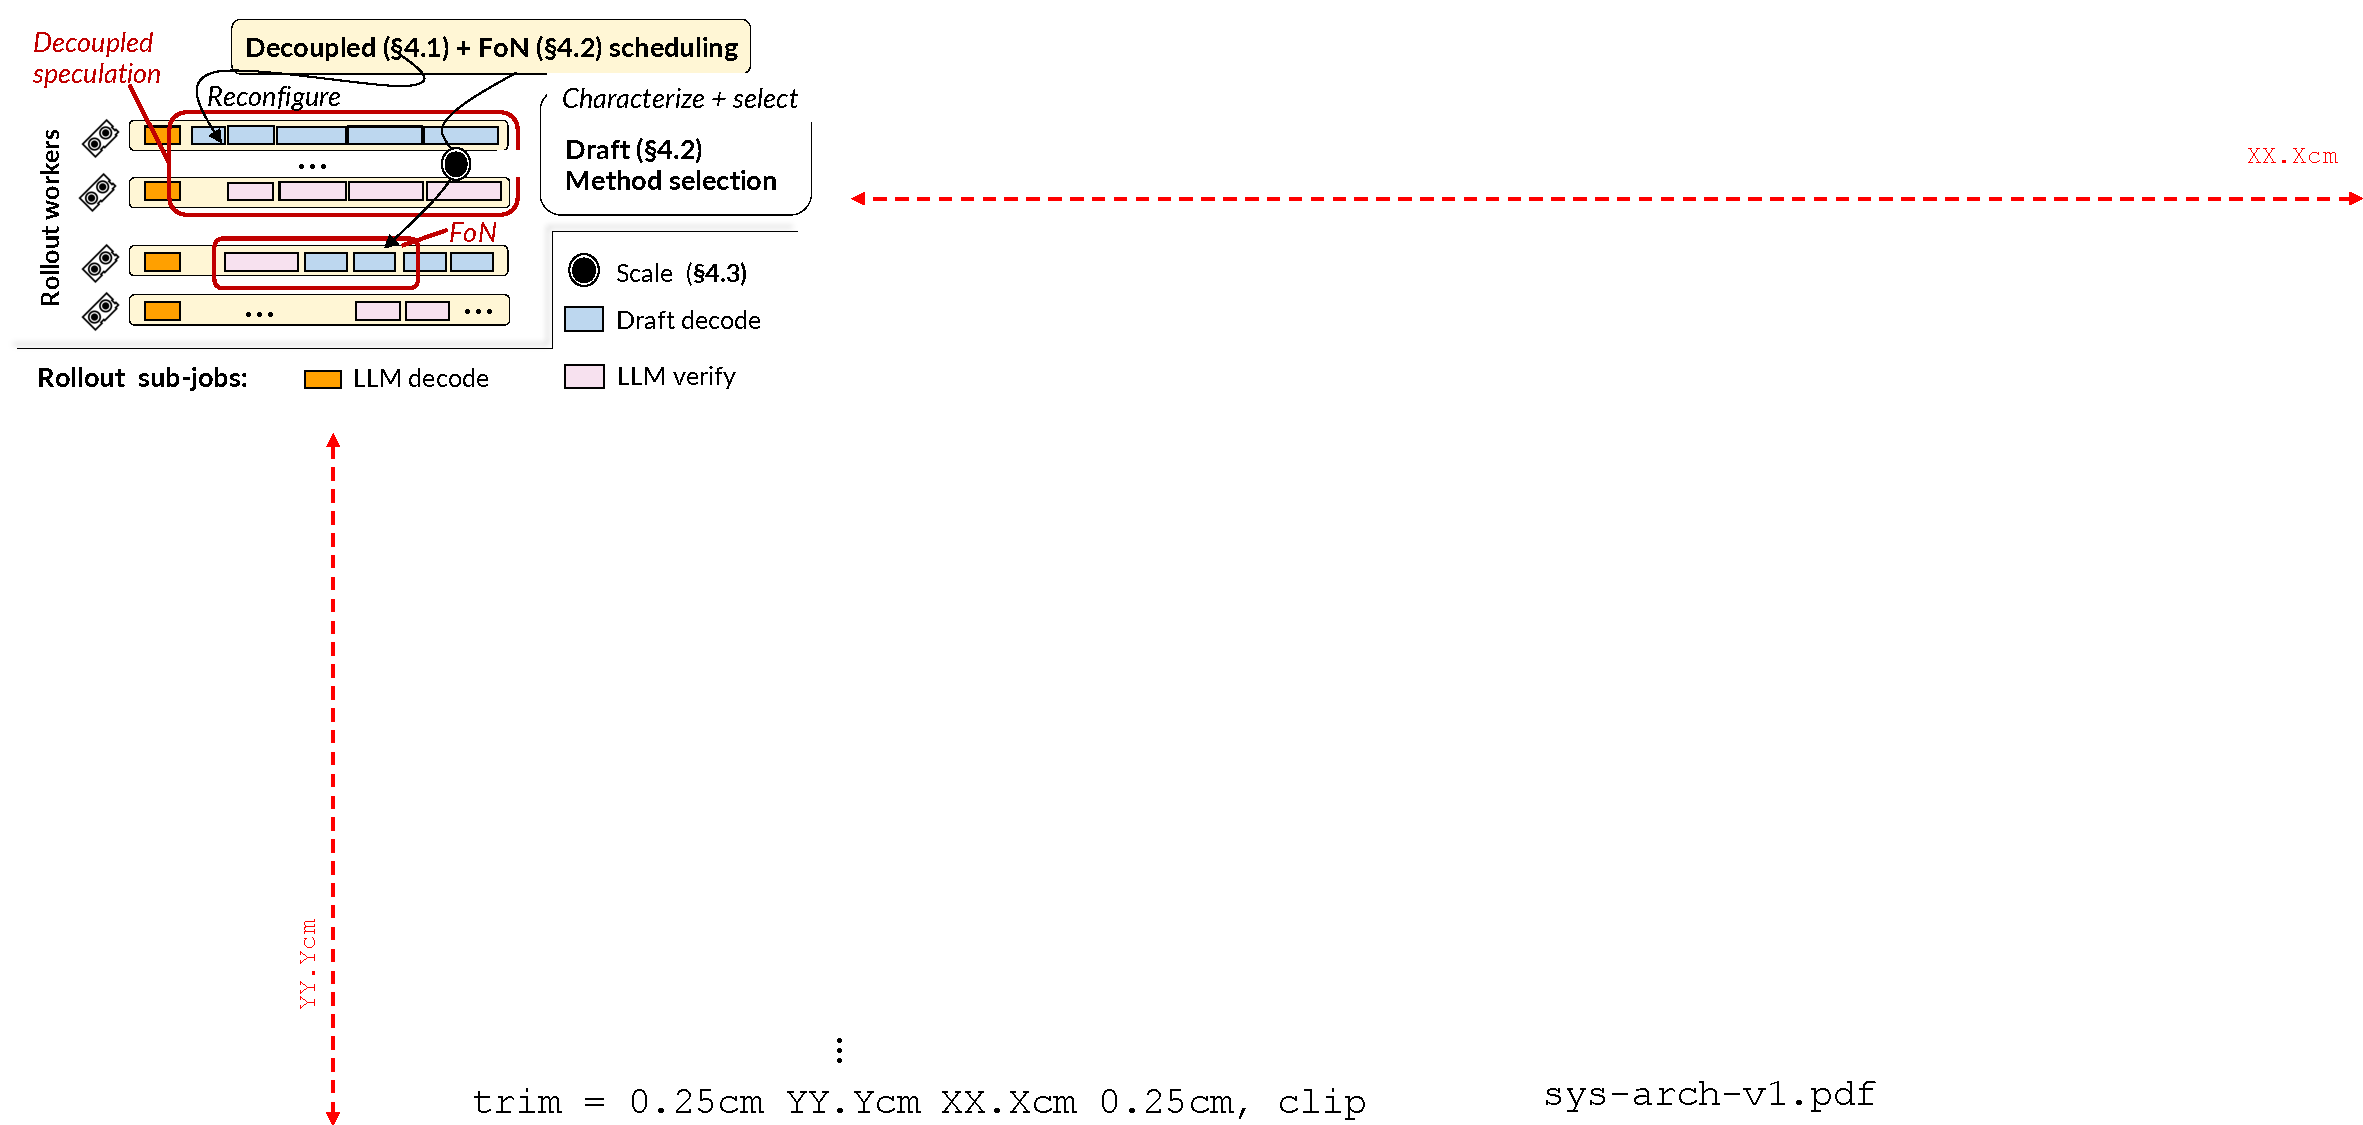
\includegraphics[width=0.95\linewidth, trim=0.25cm 12.02cm 25.63cm 0.25cm, clip]{figs/sys-arch-v1.pdf} 
        \end{minipage} \\[2pt]
        \begin{minipage}{1\linewidth}
        \caption{\small{%
            The system architecture of {\sys}.
        }}
        \label{fig:syc-arch}
        \end{minipage} \\[-15pt]
        \end{figure}  

\stitle{System architecture. \,}
{\fig{fig:syc-arch}} shows the system architecture of {\sys}:
a global scheduler searches an efficient decoupled
speculation plan (\textsection{\ref{sec:design-decouple}}) during the initial
rollout phase.
Each worker dynamically reconfigures the 
execution plan for low-acceptance-rate requests at runtime to improve efficiency.
The global scheduler monitors the GPU usage across workers to deploy 
additional draft methods for long-tailed requests
(\textsection{\ref{sec:design-bon}}).
Our runtime (\textsection{\ref{sec:design-mechanisms}}) efficiently supports
scaling primitives required for Fastest-of-N speculation. 
